\documentclass[aspectratio=169, usepdftitle=false, xcolor={dvipsnames}, 9pt]{beamer}

\usetheme[english, notoc, coloraccent=blue]{awesome}

\title{Méthodes pour l'évaluation de l'activité cyclonique tropicale en changement climatique}
\author[William]{William Dulac}
\subtitle{Soutenance de thèse}
\email{william.dulac@meteo.fr}
\institute{Centre National de Recherches Météorologiques}
\uni{Université Paul Sabatier -- Toulouse III} 
\location{Toulouse}
\date{20 Décembre 2023}

\supervisors{Julien Cattiaux, Fabrice Chauvin}
\reporters{Jean-Philippe Duvel, Sylvie Malardel}
\examinators{Jean-Pierre Chaboureau, Christophe Menkes,\par\hspace*{16ex}Caroline Muller}

\background{include/Bolaven_2023-10-11_2300Z.jpg}

\usefonttheme[onlymath]{serif}

%\setlength\abovecaptionskip{-1pt}

\addbibresource{references.bib}

\begin{document}

\maketitle

%=========================================================
\section[Introduction]{Introduction : Cyclones tropicaux}

\makesecslide

\subsection{Définition}

\begin{frame}[c]
    \frametitle{Qu'est-ce qu'un cyclone tropical ?}
    \framesubtitle{Définition et ordres de grandeur}
    \begin{columns}
        \begin{column}{0.5\textwidth}
            
        \end{column}
        \begin{column}{0.5\textwidth}
            
        \end{column}
    \end{columns}
\end{frame}

\begin{frame}[c]
    \frametitle{Qu'est-ce qu'un cyclone tropical ?}
    \framesubtitle{Le phénomène météorologique le plus destructeur}
    \begin{definition}
        \footnotesize
        \begin{itemize}
            \item Plus de 400 000 morts et près de 300 000 blessés entre 1980 et 2009 \parencite{doocy_human_2013}.
            \item 20 millions de personnes rendues sans-abri \parencite{doocy_human_2013}.
            \item Coût économique moyen de plus de 20 milliards de dollars par cyclone (TC) aux États-Unis \parencite{smith_billiondollar_2020}.
        \end{itemize} 
    \end{definition}
    \begin{columns}
        \begin{column}{0.45\textwidth}
            \begin{figure}[h]
                \centering
                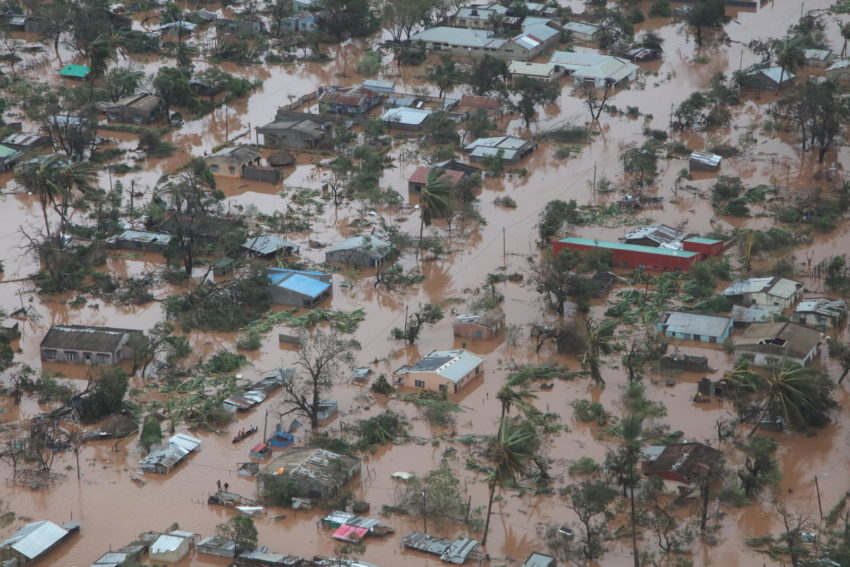
\includegraphics[width=0.97\textwidth]{Figures/idai_2019_sofala_province.jpg}
                \caption{Povince de Sofala au Mozambique après le passage du \mbox{cyclone} Idai, Mars 2019. Photo de l'Institut National
                de Gestion des Catastrophes du Mozambique (INGC).}
            \end{figure}
        \end{column}
        \begin{column}{0.45\textwidth}
             \begin{figure}[h]
                 \centering
                 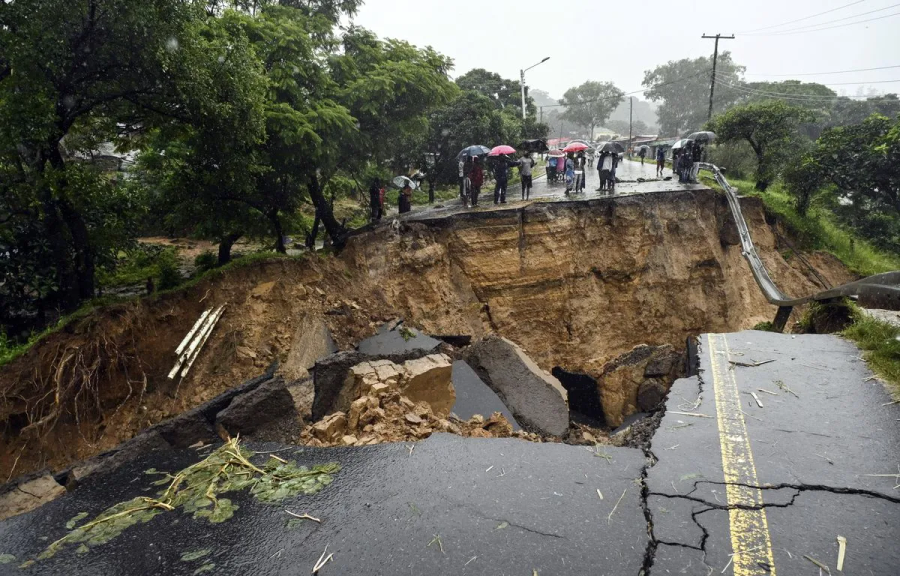
\includegraphics[width=\textwidth]{Figures/freddy_malawi_route.png}
                 \caption{Route endommagée au Malawi après le passage du cyclone Freddy, Mars 2023.\\Photo AP/SIPA/Thoko Chikondi}
             \end{figure}
        \end{column}
    \end{columns}
\end{frame}

\subsection{Consensus sur les projections futures}

\begin{frame}[c]
    \frametitle{Consensus sur l'évolution future de l'activité cyclonique}
    \begin{columns}
        \begin{column}{0.75\textwidth}
            \begin{figure}[h]
                \centering
                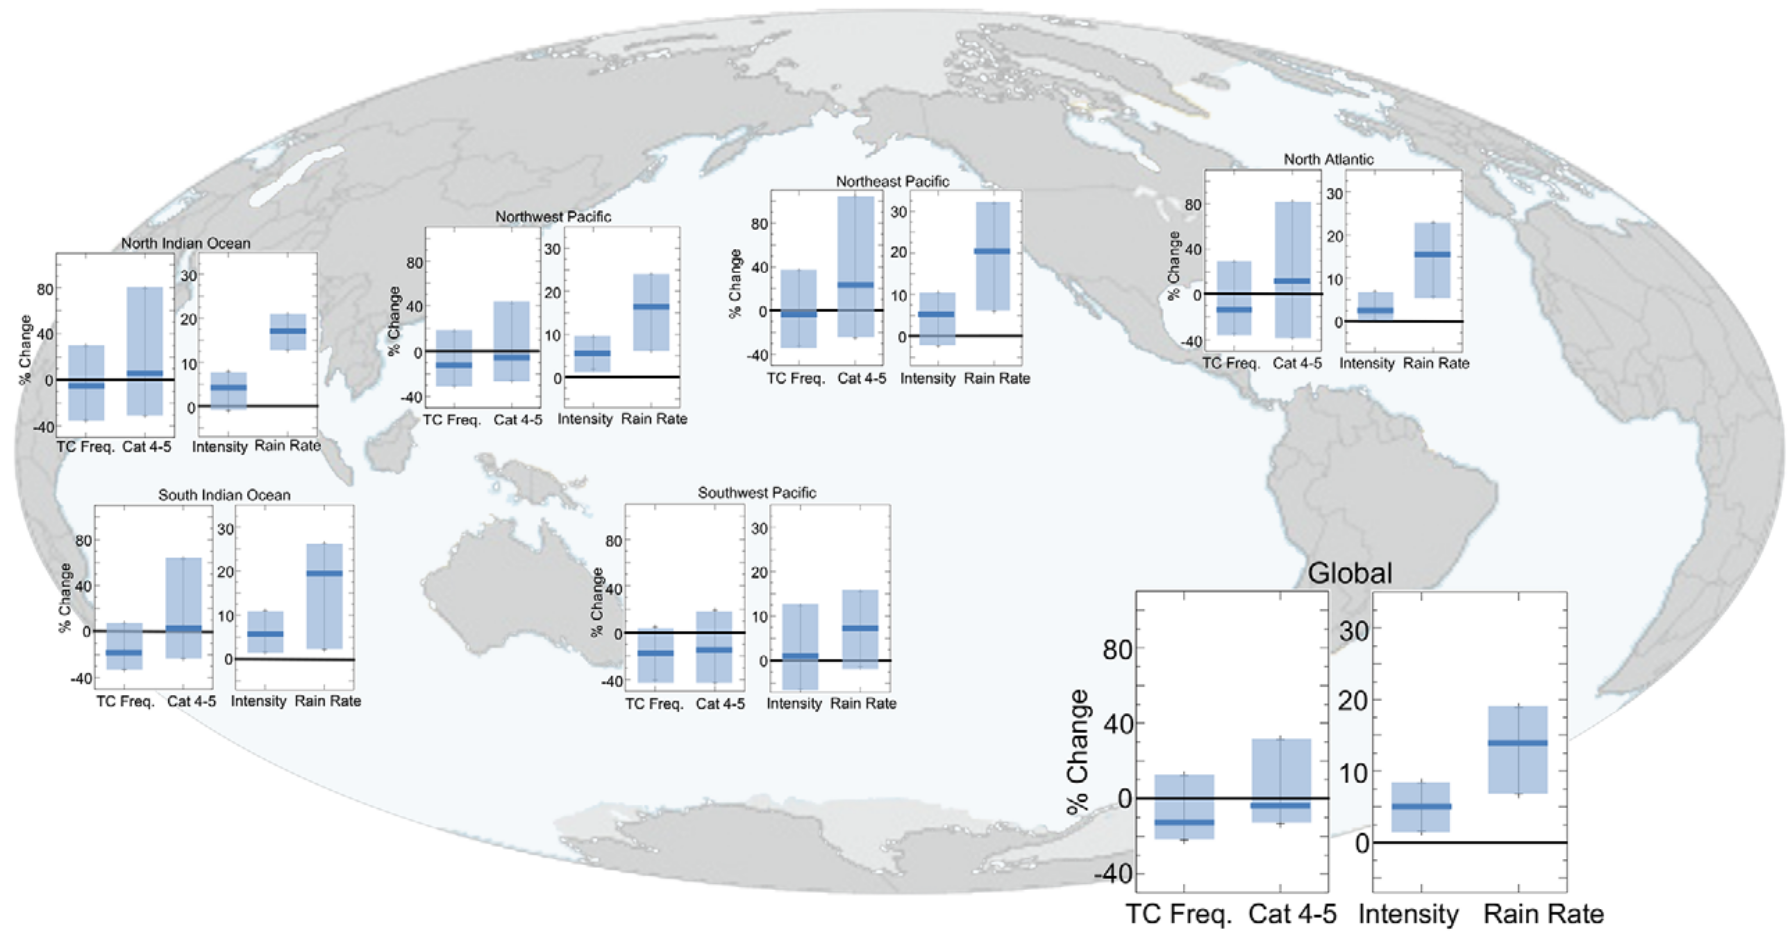
\includegraphics[width=\textwidth]{Figures/knutson_2020_projections_cropped.png}
                \caption{Synthèse des projections de l'activité cyclonique pour un réchauffement de 2°C par rapport à 1986 -- 2005
                \parencite{knutson_tropical_2020}. Médianes et intervalles de confiance de respectivement 90~\% et 80~\% (gauche et droite).}
            \end{figure}
        \end{column}
        \begin{column}{0.25\textwidth}
           \footnotesize
           \setlength{\leftmargini}{2.5ex}
           \begin{block}[Résumé]
               \scriptsize
               \begin{itemize}
                    \item Baisse probable de la fréquence en général 
                    \item Hausse probable de la fréquence des cyclones forts
                    \item Hausse fortement de l'intensité maximale
                    \item Hausse très fortement probable des précipitations
               \end{itemize}
           \end{block}
           %\pause
           %\begin{alertblock}[Limitation]
           %     \scriptsize
           %     Incertitudes sur le signe du changement, à l'échelle globale comme régionale
           %\end{alertblock}
        \end{column}
    \end{columns}
\end{frame}

\subsection[Méthodologies]{Comment sont réalisées ces projections ?}
\makesubsecslide

\begin{frame}[c]
    \frametitle{Les modèles de climat}
    \framesubtitle{Simulation numérique de l'évolution de l'état de l'atmosphère}
    \begin{columns}
        \begin{column}{0.5\textwidth}
            
        \end{column}
        \begin{column}{0.5\textwidth}
            \begin{figure}[t]
                \centering
                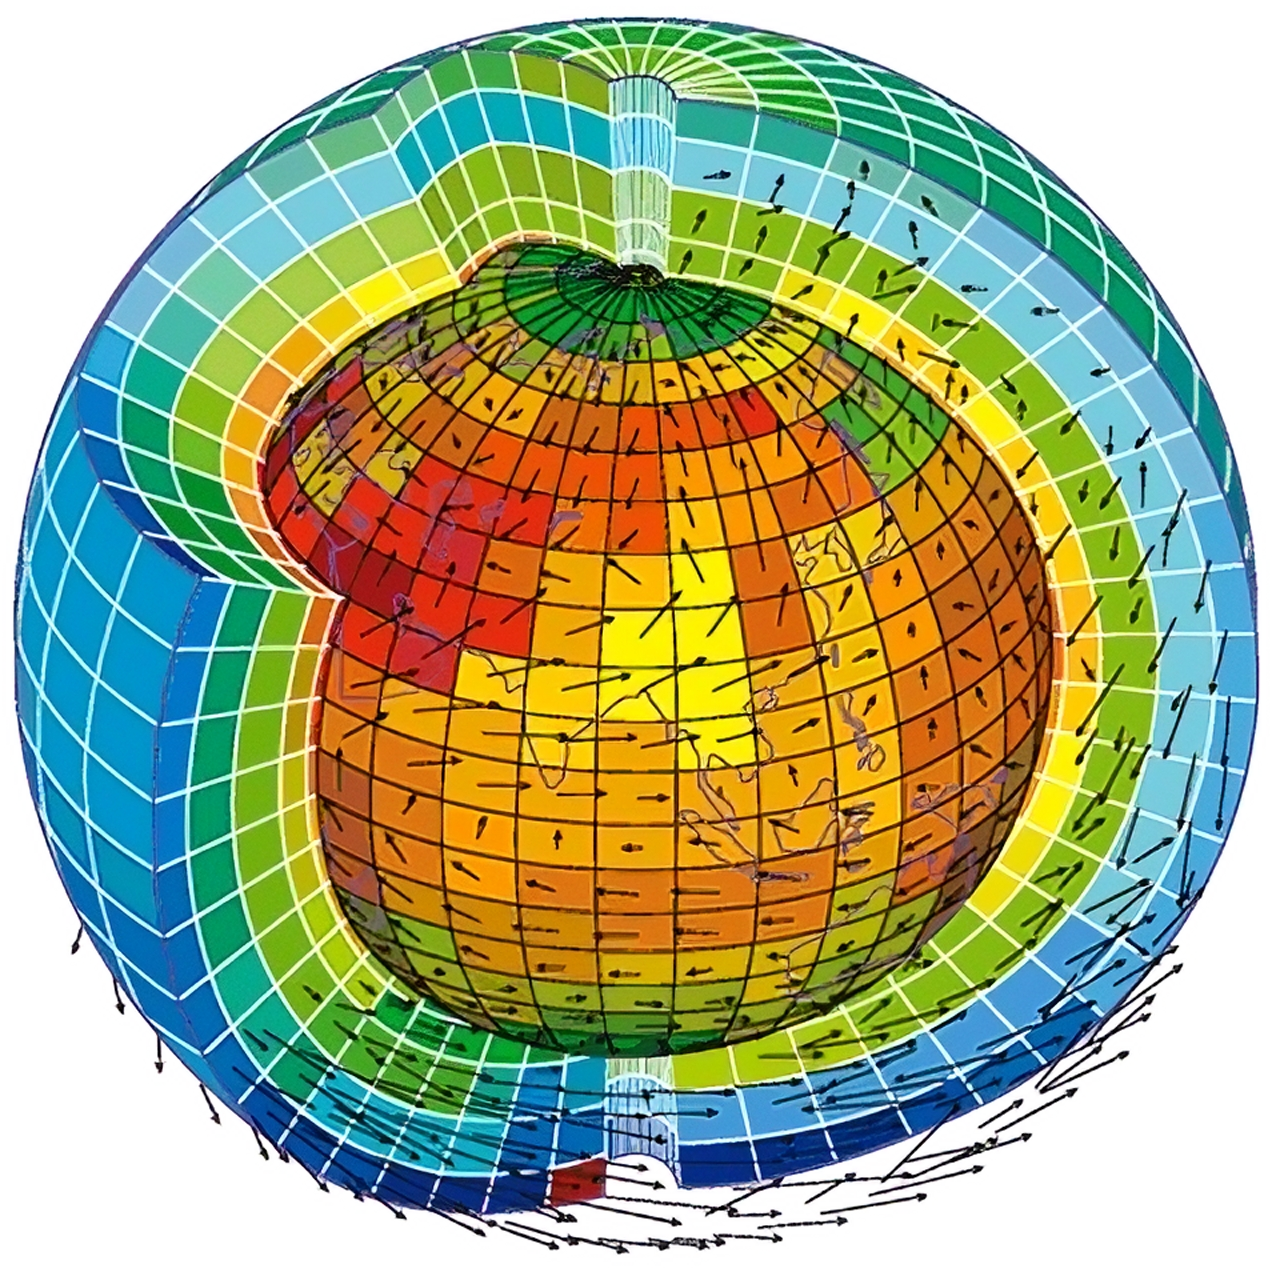
\includegraphics[width=0.8\textwidth]{Figures/maillage_upscaled_x4_2.png}
                \caption{Illustration schématique du maillage tridimensionnelle d'un modèle de climat. Les couleurs représentent la température et les flèches
                le vent.\\Illustration de \mbox{Laurent Fairhead/LMD/CNRS}.}
            \end{figure}
        \end{column}
    \end{columns} 
\end{frame}

\section{Test}

\begin{frame}[t]
    \frametitle{Plan}
    \tableofcontents[currentsection]
\end{frame}

\begin{frame}[c]
    \frametitle{Avec juste un bloc}
    \framesubtitle{Voyons voir ce que ça donne}
    
    \begin{examples}[Test]
       Ceci est un bloc 
    \end{examples}
\end{frame}

\section{Test 2}

\begin{frame}[c]
    \frametitle{Avec des listes...}
    
    \begin{columns}
        \begin{column}{0.5\textwidth}
            \begin{itemize}
                \item Foo
                \item Bar
            \end{itemize}
        \end{column}
        \begin{column}{0.5\textwidth}
           \begin{enumerate}
               \item Alpha
               \item Beta
           \end{enumerate} 
        \end{column}
    \end{columns}
\end{frame}

\end{document}
